%**********************************************
%Choose appropriate document class:

%For B.Tech ==> \documentclass[BTech]{iiitdmdiss}
%For DD ==> \documentclass[DD]{iiitdmdiss}
%For M.Tech ==> \documentclass[MTech]{iiitdmdiss}

%**********************************************
\documentclass[MTech, hidelinks]{iiitdmdiss}
%\documentclass[DD]{iiitdmdiss}
% \documentclass[BTech]{iiitdmdiss}
\usepackage{times}
\usepackage{tikz}
\usepackage{t1enc}
\usepackage[utf8]{inputenc}
\usepackage{multicol}
\usepackage{multirow}
\usepackage{pgfplots}
\usepackage{graphicx}
\usepackage{epstopdf}
\usepackage{fancyhdr}
\usepackage[driverfallback=dvipdfm]{hyperref} % hyperlinks for references.
\usepackage{amsmath} % easier math formulae, align, subequations \ldots

\usepackage{booktabs}

\renewcommand{\headrulewidth}{1pt}
\renewcommand{\footrulewidth}{1pt}

\begin{document}


%%%%%%%%%%%%%%%%%%%%%%%%%%%%%%%%%%%%%%%%%%%%%%%%%%%%%%%%%%%%%%%%%%%%%%
% Title page
%-----------------------------------------------
% Provide all the necessary information here
%-----------------------------------------------
\title{Gender classification using GAIT}
\author{Vimalraj S, E S Sarveswara Rao}
\roll{CS23M1007, CS23M1008}
% \author{Vimalraj S}
% \roll{CS23M1007}
% \author{E S Sarveswara Rao}
% \roll{CS23M1008}
\monthyear{MAY 2024}
\department{Computer Science and Engineering with specialization in Data Science and AI}
\guide{Dr. Rahul Raman}
\guidedesignation{Assistant Professor}
\guidedept{Computer Science and Engineering}
\date{15.05.2024}

%\nocite{*}
\maketitle

%%%%%%%%%%%%%%%%%%%%%%%%%%%%%%%%%%%%%%%%%%%%%%%%%%%%%%%%%%%%%%%%%%%%%%
% Declaration of originality
\declaration

%%%%%%%%%%%%%%%%%%%%%%%%%%%%%%%%%%%%%%%%%%%%%%%%%%%%%%%%%%%%%%%%%%%%%%

% Certificate
\certificate
%%%%%%%%%%%%%%%%%%%%%%%%%%%%%%%%%%%%%%%%%%%%%%%%%%%%%%%%%%%%%%%%%%%%%%

% Abstract
\abstract

Gender classification is in high demand because of its
versatility. It can be used as a surveillance system for security. It
can also be used to classify customers in retail establishments. In
this work, we propose a new gender classification technique from
a gait silhouette using observation angle-based GEIs. The system
consists of two main parts: the observation angle classification
model and the gender classification model. The observation angle
classification generates 10 observation angle-based GEIs. The
gender classification model uses angle-based GEIs to predict
gender. The proposed methods perform well with freestyle walks
which contain a viewpoint issue.
\\
\vspace{10pt}
\noindent KEYWORDS: \hspace*{0.5em} \parbox[t]{4.4in}{Gender classification, Gait, Gender recognition, GEI, CNN, Freestyle Walk}


\pagebreak

%%%%%%%%%%%%%%%%%%%%%%%%%%%%%%%%%%%%%%%%%%%%%%%%%%%%%%%%%%%%%%%%%
% Table of contents etc.

\begin{singlespace}
\tableofcontents
\thispagestyle{empty}

\listoftables
\addcontentsline{toc}{chapter}{LIST OF TABLES}
\listoffigures
\addcontentsline{toc}{chapter}{LIST OF FIGURES}
\end{singlespace}


%%%%%%%%%%%%%%%%%%%%%%%%%%%%%%%%%%%%%%%%%%%%%%%%%%%%%%%%%%%%%%%%%%%%%%
% Abbreviations
\abbreviations

\noindent 
\begin{tabbing}
xxxxxxxxxxx \= xxxxxxxxxxxxxxxxxxxxxxxxxxxxxxxxxxxxxxxxxxxxxxxx \kill
\textbf{GEI}   \> Gait Energy Image\\
\textbf{CNN}   \> Convolutional Neural Network\\

\end{tabbing}

\pagebreak

%%%%%%%%%%%%%%%%%%%%%%%%%%%%%%%%%%%%%%%%%%%%%%%%%%%%%%%%%%%%%%%%%%%%%%
% Notation

\notation
\noindent
\begin{singlespace}
\begin{tabbing}
xxxxxxxxxxx \= xxxxxxxxxxxxxxxxxxxxxxxxxxxxxxxxxxxxxxxxxxxxxxxx \kill
\textbf{$\lambda$}  \> wavelength \\

\end{tabbing}
\end{singlespace}

\pagebreak
\clearpage

% The main text will follow from this point so set the page numbering
% to arabic from here on.
\pagenumbering{arabic}
\pagestyle{fancy}
\fancyhf{}

%%%%%%%%%%%%%%%%%%%%%%%%%%%%%%%%%%%%%%%%%%%%%%%%%%%
%Enter the details of roll number, department and year for Header and Footer
%%%%%%%%%%%%%%%%%%%%%%%%%%%%%%%%%%%%%%%%%%%%%%%%%%%
\fancyhead[l]{\leftmark}
\fancyfoot[r]{\thepage}
\fancyhead[r]{CS23M1007, CS23M1008}
\fancyfoot[l]{Department of CSE, IIITDM Kancheepuram, May 2024}

%%%%%%%%%%%%%%%%%%%%%%%%%%%%%%%%%%%%%%%%%%%%%%%%%%

\chapter{INTRODUCTION}
\graphicspath{{Chapter1/}}

\section{Gender Classification}
\subsection{Existing approaches}
Gender is an important fundamental attribute of humans. Nowadays, most gender recognition methods are based on facial features. This does not perform well when the subject is far away from cameras. And when the resolution of the cameras is low.

\subsection{Using Gait}
So in order to overcome the above discussed issues, we are using GAIT analyses in order to find the gender of a human.

\section{Gait Analysis}
Gait analysis, the study of human walking patterns, has become a useful bio metric technique for identification and recognition tasks. One important gait representation called Gait Energy Images (GEIs) has gained popularity. GEIs are averaged silhouette images over a full gait cycle that capture a person's gait pattern in a compact image. 

However, GEIs are typically captured from a lateral side view, which may not always be possible in real-world scenarios. This has led to research into generating GEIs from arbitrary viewing angles to make the approach more practical.

Gender classification from gait is an important preliminary task that can improve the performance of subsequent identification systems. This project proposes a method to accurately classify an individual's gender based solely on their gait patterns captured from any viewing angle using GEIs.

The proposed approach combines the strengths of GEIs in representing gait with advanced machine learning techniques to achieve accurate gender classification from certain observation angles.

\chapter{DATASET AND PREPROCESSING}
\graphicspath{{Chapter2/}}

\section{Dataset}

Many gait datasets are available like CASIA, OU-ISIR. For our project we have used CASIA-B Gait silhouette images as input.

\subsection{CASIA-B}
Dataset B[1] is a large multi view gait database. It is Created in January 2005. There are 124 subjects (93 males, 31 females). Gait data was captured from 11 views. Three variations, namely view angle, clothing and carrying condition changes, are separately considered. Human silhouettes extracted from video files are also available.\cite{shiqi2006}

\section{Preprocessing}

\subsection{Gait Energy Image (GEI)}

After categorizing silhouette images of a walk into 11 groups, the silhouette images in the same group (except the rejected group) are combined to form 10 GEIs. For each GEI, its value at position (x, y) is defined by;

$$ GEI(x, y) = \sum_{t=1}^{n} I_t(x, y) $$

where N is the number of silhouette images in a group, It (x, y) is the value at position (x, y) of the tth image in the group.
\begin{figure}[ht]
    \centering
    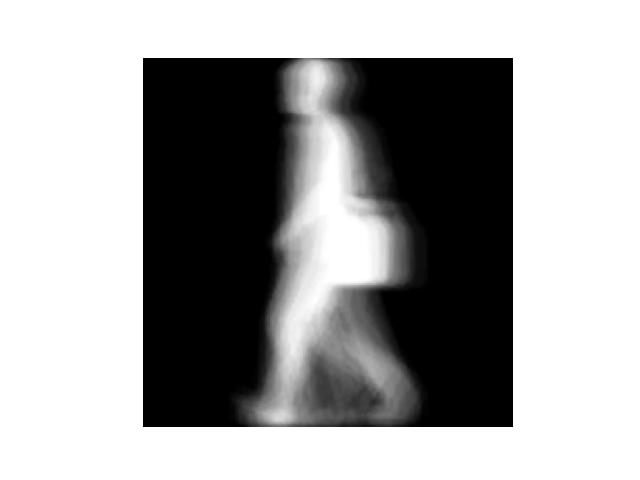
\includegraphics[scale=0.6]{data/gei.png}
    \caption{Gait Energy Image}
    \label{fig:gei}
\end{figure}

\subsection{Multi channel GEI}
Multi-channel GEI involves extracting features from the multi-dimensional gait data. This often involves calculating the covariance matrices of the data from each sensor/channel and then finding the eigenvectors and eigenvalues of these matrices. These eigenvectors represent the principal components of variation in the gait data, while the eigenvalues indicate the significance of each component.\cite{kitchat2019}

\begin{figure}[ht]
    \centering
    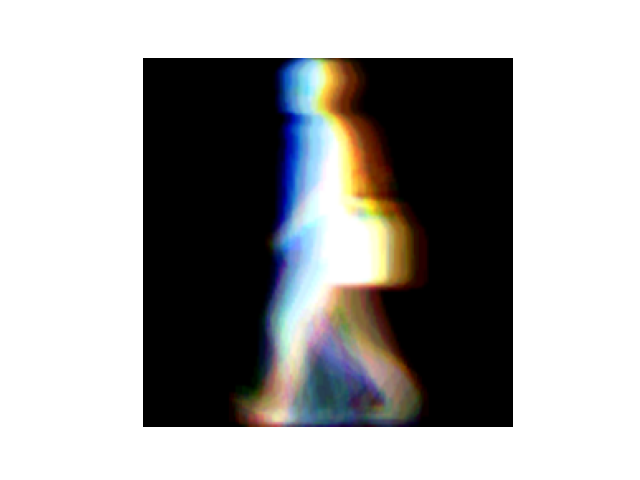
\includegraphics[scale=0.6]{data-3/gei3.png}
    \caption{3-channel GEI}
    \label{fig:gei-3}
\end{figure}

\chapter{TRAINING}
\graphicspath{{Chapter3/}}

\section{Model}

A simple Convolutional Neural Network (CNN) with the following
layers are used

\begin{itemize}
    \item Input layer of size 224 x 224
    \item 4 blocks of Convolution, ReLU, MaxPooling
    \item 2 Dense layers using ReLU activation
    \item Output layer using Sigmoid activation
\end{itemize}

\subsection{Convolution Layer}
The convolutional layer is the core building block of a CNN, and it is where the majority of computation occurs. It requires a few components, which are input data, a filter, and a feature map. Let’s assume that the input will be a color image, which is made up of a matrix of pixels in 3D. This means that the input will have three dimensions — a height, width, and depth—which correspond to RGB in an image. We also have a feature detector, also known as a kernel or a filter, which will move across the receptive fields of the image, checking if the feature is present. This process is known as a convolution.

The feature detector is a two-dimensional (2-D) array of weights, which represents part of the image. While they can vary in size, the filter size is typically a 3x3 matrix; this also determines the size of the receptive field. The filter is then applied to an area of the image, and a dot product is calculated between the input pixels and the filter. This dot product is then fed into an output array. Afterwards, the filter shifts by a stride, repeating the process until the kernel has swept across the entire image. The final output from the series of dot products from the input and the filter is known as a feature map, activation map, or a convolved feature.

Note that the weights in the feature detector remain fixed as it moves across the image, which is also known as parameter sharing. Some parameters, like the weight values, adjust during training through the process of back propagation and gradient descent. However, there are three hyper parameters which affect the volume size of the output that need to be set before the training of the neural network begins. These include:

1. The number of filters affects the depth of the output. For example, three distinct filters would yield three different feature maps, creating a depth of three. 

2. Stride is the distance, or number of pixels, that the kernel moves over the input matrix. While stride values of two or greater is rare, a larger stride yields a smaller output.

3. Zero-padding is usually used when the filters do not fit the input image. This sets all elements that fall outside of the input matrix to zero, producing a larger or equally sized output. There are three types of padding:
         Valid padding: This is also known as no padding. In this case, the last convolution is dropped if dimensions do not align.
    
         Same padding: This padding ensures that the output layer has the same size as the input layer.
    
         Full padding: This type of padding increases the size of the output by adding zeros to the border of the input.

After each convolution operation, a CNN applies a Rectified Linear Unit (ReLU) transformation to the feature map, introducing nonlinearity to the model.

\subsection{Relu Activation}
The rectified linear unit (ReLU) or rectifier activation function introduces the property of non linearity to a deep learning model and solves the vanishing gradients issue. It interprets the positive part of its argument. It is one of the most popular activation functions in deep learning.

The ReLU Function is given as, \[f(x) = max(0,x)\]

\subsection{Max Pooling Layer}
Max pooling is a downsampling technique commonly used in convolutional neural networks (CNNs) to reduce the spatial dimensions of an input volume. It is a form of non-linear down-sampling that serves to make the representation smaller and more manageable, and to reduce the number of parameters and computation in the network. Max pooling operates independently on each depth slice of the input and resizes it spatially.

The primary objective of max pooling is to reduce the amount of information in an image while maintaining the essential features necessary for accurate image recognition. This process helps to make the detection of features in input data invariant to scale and orientation changes and also aids in preventing overfitting.

\subsection{Fully connected layers}
A fully connected layer refers to a neural network in which each neuron applies a linear transformation to the input vector through a weights matrix. As a result, all possible connections layer-to-layer are present, meaning every input of the input vector influences every output of the output vector.

\subsection{Sigmoid Activation}
Sigmoid function is as the activation for the output layer of binary classification models. It squashes the output to a probability value between 0 and 1, which can be interpreted as the probability of the input belonging to a particular class.

The Sigmoid Function is given as, \[f(x) = \frac{1} {1+e^{-x}}\]



\subsection{Loss Function}

Binary Cross Entropy is a loss function used in machine learning and deep learning to measure the difference between predicted binary outcomes and actual binary labels. It quantifies the dissimilarity between probability distributions, aiding model training by penalizing inaccurate predictions. It’s widely used in tasks like binary classification, where the goal is to categorize data into two classes.

\[ Loss = \frac{-1}{N} * \sum_{i=1}^{N} yi * log(pi) + (1-yi) * log(1-pi) \]

Binary Cross Entropy, also known as Binary Log Loss or Binary Cross-Entropy Loss, is a commonly used loss function in machine learning, particularly in binary classification problems. It is designed to measure the dissimilarity between the predicted probability distribution and the true binary labels of a dataset.

\section{Training}

The CNN model is trained separately for 5 different angles: 90 degrees, 72 degrees, 54 degrees, 36 degrees, and 18 degrees.

The models are trained using two types of input data:
\begin{itemize}
    \item GEI (Gait Energy Image)
    \item 3-channel GEI
\end{itemize}

The only difference between the two inputs is the number of channels - GEI is a single-channel image, while 3-channel GEI has 3 color channels. So the model also differs only at the Input Layer.

\subsection{Training History}
\begin{figure}[ht]
    \centering
    \includegraphics[width=\textwidth]{data/nm-90.png}
    \caption{Training history for 90 degrees}
    \label{fig:nm-90}
\end{figure}

\begin{figure}[ht]
    \centering
    \includegraphics[width=\textwidth]{data/nm-72.png}
    \caption{Training history for 72 degrees}
    \label{fig:nm-72}
\end{figure}

\begin{figure}[ht]
    \centering
    \includegraphics[width=\textwidth]{data/nm-54.png}
    \caption{Training history for 54 degrees}
    \label{fig:nm-54}
\end{figure}

\begin{figure}[ht]
    \centering
    \includegraphics[width=\textwidth]{data/nm-36.png}
    \caption{Training history for 36 degrees}
    \label{fig:nm-36}
\end{figure}

\begin{figure}[ht]
    \centering
    \includegraphics[width=\textwidth]{data/nm-18.png}
    \caption{Training history for 18 degrees}
    \label{fig:nm-18}
\end{figure}

% for 3 channel GEI

\begin{figure}[ht]
    \centering
    \includegraphics[width=\textwidth]{data-3/nm-90.png}
    \caption{Training history for 90 degrees, 3-channel GEI}
    \label{fig:nm-90-3}
\end{figure}

\begin{figure}[ht]
    \centering
    \includegraphics[width=\textwidth]{data-3/nm-72.png}
    \caption{Training history for 72 degrees, 3-channel GEI}
    \label{fig:nm-72-3}
\end{figure}

\begin{figure}[ht]
    \centering
    \includegraphics[width=\textwidth]{data-3/nm-54.png}
    \caption{Training history for 54 degrees, 3-channel GEI}
    \label{fig:nm-54-3}
\end{figure}

\begin{figure}[ht]
    \centering
    \includegraphics[width=\textwidth]{data-3/nm-36.png}
    \caption{Training history for 36 degrees, 3-channel GEI}
    \label{fig:nm-36-3}
\end{figure}

\begin{figure}[ht]
    \centering
    \includegraphics[width=\textwidth]{data-3/nm-18.png}
    \caption{Training history for 18 degrees, 3-channel GEI}
    \label{fig:nm-18-3}
\end{figure}


\chapter{EVALUATION AND COMPARISON}
\graphicspath{{Chapter4/}}

\section{Evaluation Metrics}
\subsection{Confusion Matrix}
For the gender classification from gait using observation angle-based GEIs project, the confusion matrix will be a valuable metric to evaluate the performance of the proposed method. A confusion matrix provides a comprehensive breakdown of the classification results, allowing for a detailed analysis of the model's accuracy and potential errors.

In the context of this binary classification task (male or female), the confusion matrix will be a 2x2 table that summarizes the counts of true positives (TP), true negatives (TN), false positives (FP), and false negatives (FN). The rows of the matrix represent the actual classes (male or female), while the columns represent the predicted classes.

The confusion matrix will provide the following information:
\begin{itemize}
    \item True Positives
    \item True Negatives
    \item False Positives
    \item False Negatives
    \item Accuracy
    \item Precision
    \item Recall
    \item F1 Score
\end{itemize}
\subsection{True Positives}
The number of instances where the model correctly predicted the gender as male for actual male samples.

\subsection{True Negatives}
The number of instances where the model correctly predicted the gender as female for actual female samples.

\subsection{False Positives}
The number of instances where the model incorrectly predicted the gender as male for actual female samples.

\subsection{False Negatives}
The number of instances where the model incorrectly predicted the gender as female for actual male samples.

From the confusion matrix, several evaluation metrics can be derived to assess the performance of the proposed method:

\subsection{Accuracy}
The overall proportion of correct predictions, calculated as (TP + TN) / (TP + TN + FP + FN).

\subsection{Precision}
The proportion of true positives among all positive predictions, calculated as TP / (TP + FP) for each class.

\subsection{Recall}
The proportion of actual positives that are correctly identified, calculated as TP / (TP + FN) for each class.

\subsection{F1 Score}
The harmonic mean of precision and recall, providing a balanced measure of overall performance.

By analyzing the confusion matrix and these derived metrics, the researchers can gain insights into the strengths and weaknesses of the proposed method. They can identify specific cases where the model struggles, such as mis classifying males as females or vice versa, and potentially investigate the underlying reasons behind these errors.

Furthermore, the confusion matrix can be used to compare the performance of the proposed method with existing techniques or baseline models, allowing for a comprehensive evaluation and bench marking of the approach.

Overall, the confusion matrix will serve as a valuable tool for assessing the gender classification performance of the proposed observation angle-based GEI method, enabling the researchers to quantify and analyze the results, identify areas for improvement, and demonstrate the effectiveness of their approach.


\section{Comparison between models trained on different angles}

\begin{table}
    \centering
    \begin{tabular}{rrrrr}
\toprule
angle & accuracy & precision & recall & f1\_score \\
\midrule
90 & 0.927 & 1.000 & 0.771 & 0.871 \\
72 & 0.900 & 0.780 & 0.958 & 0.860 \\
54 & 0.833 & 0.658 & 1.000 & 0.793 \\
36 & 0.460 & 0.372 & 1.000 & 0.542 \\
18 & 0.320 & 0.320 & 1.000 & 0.485 \\
\bottomrule
\end{tabular}

    \caption{Comparison of metrics while using different angles}
    \label{fig:comp}
\end{table}

\begin{table}
    \centering
    \begin{tabular}{rrrrr}
\toprule
angle & accuracy & precision & recall & f1\_score \\
\midrule
90 & 0.927 & 1.000 & 0.771 & 0.871 \\
72 & 0.900 & 0.780 & 0.958 & 0.860 \\
54 & 0.833 & 0.658 & 1.000 & 0.793 \\
36 & 0.460 & 0.372 & 1.000 & 0.542 \\
18 & 0.320 & 0.320 & 1.000 & 0.485 \\
\bottomrule
\end{tabular}

    \caption{Comparison of metrics while using different angles, using 3-channel GEI}
    \label{fig:comp-3}
\end{table}

As shown in \ref{fig:comp} and \ref{fig:comp-3} the accuracy increases while using 3-channel GEI only at 90 degrees, stays the same at 72 degrees and decreases for all other angles.
\chapter{CONCLUSION AND FUTURE SCOPE}
\label{chap:conclusions}

\section{Conclusion}
The model trained on 90° GEI’s perform better than other models. Using 3-channel GEI’s improve accuracy only at 90 degrees. 90° is the ideal angle to capture gait, but even for 72° gait sequence
the model gives accuracy around 90%.

\section{Future Scope}
This approach can be extended to perform different types of classification. This simple model achieves good accuracy for the binary classification task. Other complex models may be required to extract features in a multi class classification problem.

%%%%%%%%%%%%%%%%%%%%%%%%%%%%%%%%%%%%%%%%%%%%%%%%%%%%%%%%%%%%
% Bibliography.

\begin{singlespace}
  \bibliography{References}
\end{singlespace}

\end{document}
